%%
%% Template LaTeX2e file
%%
\documentclass[a4paper]{article}
\usepackage{german,color}
\usepackage[utf8]{inputenc}
\usepackage{graphicx}
\usepackage{calc}

\newcommand\SC{"`Sparmatic Comet"' }

\title {
Bedienungsanleitung Alternativ-Fimrware für \SC
}

\author {
\sf Jörg Wunsch
}

%% if you wanna set a specified date:
%\date {
%25-Mar-88
%}

\sloppy

\begin {document}

\maketitle

%%\tableofcontents

\section {
Beschreibung der Hardware
}

Die Hardware des \SC besteht aus einem Gehäuse, welches auf einen auf
das eigentliche Heizkörperventil geschraubten Polyethylen-Ring
aufgeschnappt wird.  Um das Gehäuse wieder von diesem Ring zu lösen,
betätigt man auf der Unterseite eine kleine Drucktaste.

Auf der Oberseite des Gehäuses befindet sich ein LC-Display, darunter
drei Tasten sowie ein Stellknopf.

Die Frontseite des Gehäuses beherbergt unter einer kleinen Abdeckung zwei
Batterien der Größe LR6.

\subsection {
  Das LC-Display
}

Das LC-Display gliedert sich in mehrere Bereiche bzw. Elemente, die in
Bild \ref{LCD} dargestellt sind.

\begin{figure}[h]
\centering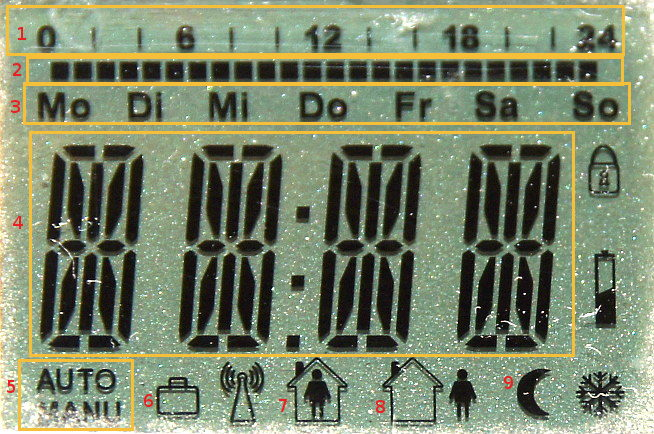
\includegraphics[width=0.5\linewidth]{LCD.jpg}
\caption{Elemente des LC-Displays}
\label{LCD}
\end{figure}

Im Einzelnen handelt es sich dabei:

\begin{enumerate}
%1
\item \textbf{Stundenanzeige} Diese Anzeige bezeichnet grob die
  Stunden des darunterliegenden Anzeigebalkens.  Die Stundenanzeige
  wird beim Start der Firmware aktiviert und dient daher als
  Einschaltanzeige.
%2
\item \textbf{Anzeigebalken} Der Anzeigebalken beschreibt im
  Automatikmodus bzw. während der Programmiermenüs für den
  Automatikmodus die Stunden des Tages, während derer die "`zu
  Hause"'-Temperatur aktiv ist.  Ein Kästchen entspricht einer Stunde.
%3
\item \textbf{Wochentagsanzeige} In dieser Zeile wird der Wochentag
  angezeigt.  Im Normalzustand ist dies der aktuelle Wochentag gemäß
  der eingestellten Uhr, in den Programmierfunktionen wird dabei der
  Tag oder die Tage angezeigt, für den die Programmierung gerade
  erfolgt bzw. beim Urlaubs-Menü der Wochentag, der gerade als Ende
  des Urlaubs gewählt ist.
%4
\item \textbf{Hauptanzeige} Hier werden im Normalzustand abwechselnd
  die aktuelle Uhrzeit und die letzte gemessene Temperatur angezeigt.
  Während der Menüfunktionen wird dort ein entsprechender Menütext
  angezeigt oder der aktuell eingestellte Wert.
%5
\item \textbf{Anzeige des Betriebsmodus} Das Wort "`MANU"' wird
  angezeigt, wenn die Temperaturregelung gemäß dem manuell eingestellten
  Wert erfolgt.  Das Wort "`AUTO"' wird angezeigt, wenn das
  Temperaturprofil dem zuvor programmierten Zeitverlauf folgt.
%6
\item \textbf{Urlaubs-Symbol} Wenn dieses Symbol angezeigt wird, dann
  ist derzeit eine Urlaubsfunktion aktiv.
%7
\item \textbf{"`zu Hause"'} Wenn dieses Symbol angezeigt wird, dann
  folgt die Solltemperatur dem Wert für "`zu Hause"'.
%8
\item \textbf{"`außer Haus"'} Wenn dieses Symbol angezeigt wird, dann
  folgt die Solltemperatur dem Wert für "`außer Haus"'.
%9
\item \textbf{"`Nacht"'} Wenn dieses Symbol angezeigt wird, dann folgt
  die Solltemperatur dem Wert für "`Nachtbetrieb"'.

\end{enumerate}

\subsection {
  Tasten und Stell-Rad
}

Der Tastenblock des \SC besteht aus drei Tasten:

\begin{itemize}
\item \textbf{MENU} Diese Taste schaltet den Menü-Modus ein oder aus.
\item \textbf{OK} Diese Taste bestätigt im Menü-Modus eine bestimmte
  Einstellung oder Funktion.
\item \textbf{Uhr} Diese Taste hat derzeit keine Funktion.
\end{itemize}

Das Stell-Rad unter den Tasten erlaubt es, bestimmte Einstellungen zu
ändern oder durch die Menüs hindurch zu schalten.

Im Grundzustand wird durch dieses Rad die aktuelle Soll-Temperatur
der Regelung geändert.

\section {
  Beschreibung der Software
}

\subsection {
  Inbetriebnahme
}

Die Inbetriebnahme erfolgt durch Einlegen von 2 Batterien LR6 in das
Batteriefach.  Im Display erscheinen nach links wandernde kleine
Pfeile, die andeuten, dass der Stellmotor das Ventil maximal öffnet.
Anschließend blinkt der Text "`INST OK"'.  In diesem Zustand sollte
das Ventil auf den Heizkörper aufgesteckt werden.

Danach wird die "`OK"'-Taste betätigt, und die Firmware führt eine
Erstkalibrierung des Ventilwegs durch.

Danach sollte sinnvollerweise noch das aktuelle Datum sowie die
Uhrzeit eingetragen werden.

Das \SC befindet sich danach im manuellen Betriebsmodus.

\subsection {
  Betriebsmodi: MANU vs. AUTO
}

Im manuellen Modus wechselt
die Anzeige zwischen aktueller Uhrzeit und letzter gemessener
Temperatur.

In diesem Modus regelt die Regelung auf die eingestellte Solltemperatur.
Die Solltemperatur lässt sich mit dem Einstellrädchen ändern.

Im Automatikmodus wird die Solltemperatur für die Regelung bei jedem
Übergang zwischen den einzelnen Zuständen ("`im Haus"', "`außer Haus"'
und "`Nacht"') an die voreingestellten Werte angepasst.  Der Sollwert
kann danach wie im manuellen Modus mit dem Stell-Rad noch geändert
werden; in diesem Falle bleibt er bis zum nächsten Übergang auf einen
der voreingestellten Werte erhalten.


\end {document}

